%This is to test out tikz graph specifications


\documentclass[letterpaper, 12pt]{report}
%\usepackage[pdftex,active,tightpage]{preview}
%\setlength\PreviewBorder{2mm} % use to add a border around the image
\usepackage{tikz}
\usetikzlibrary{arrows,decorations.pathmorphing,backgrounds,positioning,fit,petri,calc,shapes}
%\usepackage[small]{caption}
%\usepackage{pdflscape}

% % % % % % % % % % % % % % % % % % % % % % %
%global tikzstyles I use in all the path diagrams
\tikzstyle{observed}=[rectangle, thick, minimum size = 10mm, draw =black!80]
\tikzstyle{latent}=[circle, thick, minimum size = 10mm, draw =black!80]
\tikzstyle{connect}=[-latex, thick]  
\tikzstyle{latent2}=[draw=none,fill=none]

\begin{document}

%Selection Effect Diagram
\begin{figure*}
\centering
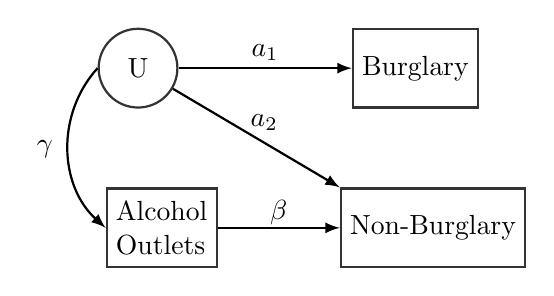
\begin{tikzpicture}[every text node part/.style={align=left}]
  \node[latent]   (U) {U};
  \node[observed] (Bar) [below=of U,xshift=3mm]{Alcohol \\ Outlets};
  \node[observed] (Bur) [right=of U,xshift=12mm]{Burglary};  
  \node[observed] (NonBu) [right=of Bar,xshift=5.5mm]{Non-Burglary};  
  
  \path (U.west) edge [connect, bend right=45] node [xshift=-3mm]{$\gamma$} (Bar.west)
        (U) edge [connect] node [yshift=2mm]{$a_1$} (Bur)
        (U) edge [connect] node [yshift=2mm,xshift=1mm]{$a_2$} (NonBu.north west)
        (Bar) edge [connect] node [yshift=2mm]{$\beta$} (NonBu);
\end{tikzpicture}
\caption{}
\label{fig:UnPath}
\end{figure*}


%\begin{table}
%\caption{Sources of Data and Characteristics they should be measuring.}
%\label{table_sources}
%\centering
%\scalebox{0.7} {
%\begin{tabular}{|l|l|l|l|l|}
%    \hline
%\textbf{Name} & \textbf{Support} & \textbf{People} & \textbf{Places} & \textbf{Opportunities} \\ \hline
%\textbf{Crime Data} & Points & & & \\
%311 Service Requests & Points &  & X &  \\ 
%Registered Vacant Property & Points &  & X &  \\ 
%Green Site & Points &  & X &  \\ 
%Trees & Points &  & X &  \\ 
%Parks & Polygon &  & X & X \\ 
%Sidewalks & Polygon &  & X &  \\ 
%Street Lighting & Points &  & X &  \\ 
%Outdoor recreational facilities & Points &  &  & X \\ 
%Litter Cans & Points &  & X &  \\ 
%Toxic Release Inventory Sites & Points &  & X &  \\ 
%Roads & Polygon &  & X &  \\ 
%Public Housing & Polygon & X & X & X \\ 
%Alcohol Licenses* & Points &  &  & X \\ 
%Places of Worship & Points &  &  & X \\ 
%Halfway Houses & Points & X &  & X \\ 
%Hospitals & Polygon &  &  & X \\ 
%Police Stations & Points &  &  & X \\ 
%Place of Worship & Points &  &  & X \\ 
%Bus Stops & Points &  &  & X \\ 
%Subway Entrances & Points &  &  & X \\ 
%Halfway House & Points & X &  &  \\ 
%HIV Clinic & Points & X &  &  \\ 
%Public Housing & Points & X &  & X \\ 
%Library & Points &  &  & X \\ 
%Schools & Polygon &  &  & X \\ 
%University Area & Polygon &  &  & X \\ 
%Recreation Area & Polygon &  &  & X \\ 
%Wireless Hot Spot & Points & X &  & X \\ 
%Shopping Centres & Points & X &  & X \\ 
%Sidwalk Caf\'e & Points & X &  & X \\ \hline
%\multicolumn{5}{l}{\tiny{*Alcohol licenses are subsequently split between types liquor stores, grocery or convenience, and bars or restaurants.}} 
%\end{tabular}
%}
%\end{table}


%\begin{preview}
%%\begin{figure}
%
%
%\begin{tikzpicture}
%    %Street Grid
%    \coordinate (LL) at (0,0);
%    \coordinate (UL) at (0,6);
%    \coordinate (ML) at (0,3);
%    \coordinate (MR) at (4,3);
%    \coordinate (LR) at (4,0);
%    \coordinate (UR) at (4,6);
%
%    %background grid
%    \draw[-, line width=2.5pt] (LL) -- (UL);
%    \draw[-, line width=2.5pt] (LR) -- (UR);
%    \draw[-, line width=2.5pt] (ML) -- (MR);
%
%    %Circles for area effects
%    \coordinate (Lo) at (2,3);
%    \filldraw [blue] (Lo) circle [radius=0.7cm]; 
%    \filldraw [orange] (LL) circle [radius=0.35cm];
%    \filldraw [orange] (UL) circle [radius=0.35cm];
%    \filldraw [orange] (ML) circle [radius=0.35cm];
%    \filldraw [orange] (LR) circle [radius=0.35cm];
%    \filldraw [orange] (UR) circle [radius=0.35cm];
%    \filldraw [orange] (MR) circle [radius=0.35cm];
%\end{tikzpicture}



%\begin{tikzpicture}
%  \node[latent2,yshift=-25mm] (Social) {Social};
%  \node[latent2] (Direct) [right=of Social, yshift=25mm]{Direct};
%  \node[latent2] (Referral) [above=of Direct,xshift=0mm]{Referral};  
%  \node[latent2] (Z) [below=of Direct]{Z};  
%  \node[latent2] (Traffic) [right=of Direct, xshift=5mm]{Traffic};
%  
%  \path (Social.north east) edge [connect] node [yshift=3mm, xshift=-2mm]{$d$} (Direct.west)
%        (Social.north) edge [connect] node [yshift=2mm, xshift=-2mm]{$r$} (Referral.west)
%        (Social.east) edge [connect] node [yshift=3mm]{$z$} (Z.west)
%        (Referral.east) edge [connect, yshift=1mm] node [yshift=3mm]{$1$} (Traffic.north west)
%        (Direct.east) edge [connect] node [yshift=3mm]{$1$} (Traffic.west)        
%        (Z.east) edge [connect, yshift=-3mm] node [yshift=3mm]{$1$} (Traffic.south west)        
%        (Social.south east) edge [connect, bend right=90] node [yshift=3mm]{$1$} (Traffic.south);
%        
%\end{tikzpicture}
%\label{fig:UnPath}

%\end{figure}
%\end{preview}
\end{document}